\documentclass[border=6pt]{standalone}
\usepackage{amsmath}
\usepackage{tikz}
\usetikzlibrary{arrows.meta}
\begin{document}
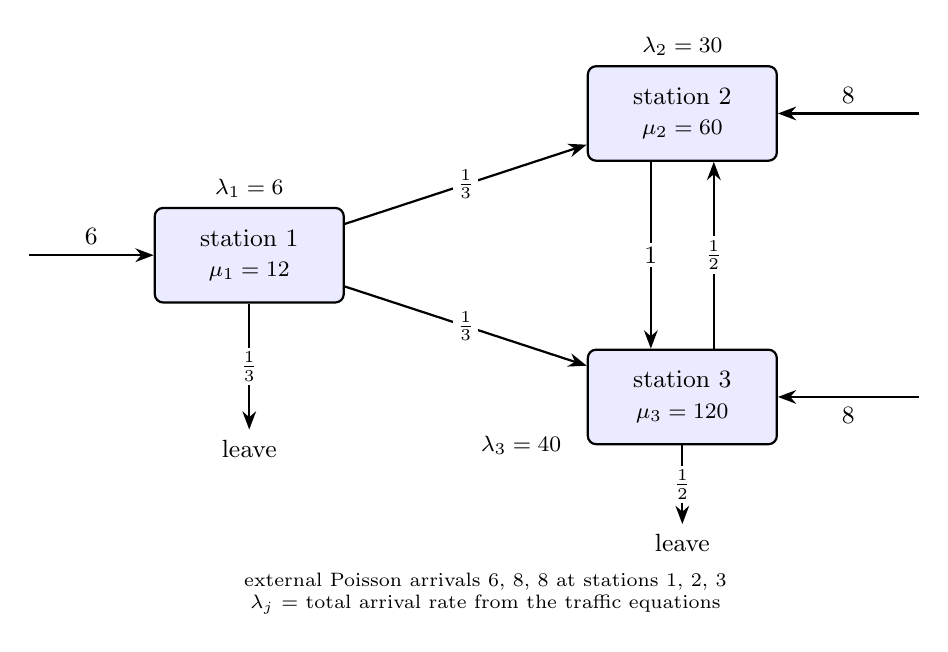
\begin{tikzpicture}[>=Stealth,font=\small,
 s/.style={draw,thick,circle,minimum size=1.1cm,inner sep=0pt,fill=blue!8},
 e/.style={->,thick},
 lab/.style={font=\small,fill=white,inner sep=1.5pt},
 every loop/.style={->,thick,looseness=6}]
\tikzset{st/.style={draw,thick,rounded corners=3pt,fill=blue!8,align=center,minimum width=2.4cm,minimum height=1.2cm}}
\node[st] (1) at (0,0) {station 1\\{\footnotesize $\mu_1=12$}};
\node[st] (2) at (5.5,1.8) {station 2\\{\footnotesize $\mu_2=60$}};
\node[st] (3) at (5.5,-1.8) {station 3\\{\footnotesize $\mu_3=120$}};
\draw[e] (-2.8,0) -- node[above]{6} (1);
\draw[e] (8.5,1.8) -- node[above]{8} (2);
\draw[e] (8.5,-1.8) -- node[below]{8} (3);
\draw[e] (1) -- node[lab]{$\tfrac13$} (2);
\draw[e] (1) -- node[lab]{$\tfrac13$} (3);
\draw[e] (1.south) -- node[lab]{$\tfrac13$} ++(0,-1.6) node[below]{leave};
\draw[e] ([xshift=-4mm]2.south) -- node[lab]{1} ([xshift=-4mm]3.north);
\draw[e] ([xshift=4mm]3.north) -- node[lab]{$\tfrac12$} ([xshift=4mm]2.south);
\draw[e] (3.south) -- node[lab]{$\tfrac12$} ++(0,-1.0) node[below]{leave};
\node[font=\footnotesize,anchor=south] at (2.north) {$\lambda_2=30$};
\node[font=\footnotesize,anchor=south] at (1.north) {$\lambda_1=6$};
\node[font=\footnotesize,anchor=east] at ([xshift=-2mm]3.south west) {$\lambda_3=40$};
\node[font=\scriptsize,align=center] at (3,-4.3) {external Poisson arrivals 6, 8, 8 at stations 1, 2, 3\\$\lambda_j$ = total arrival rate from the traffic equations};
\end{tikzpicture}
\end{document}
